\newpage\section{Introduction}

\subsection{Background and Motivation}

%Einführung Data Analytics ist wichtig
The introduction and widespread usage of computers has proven to be disruptive for all industries. Entire industrial sectors have been reshaped, whole professions made obsolete and new career opportunities have been created. This shift towards the adaption of \ac{it} has been necessary for businesses to stay competitive in the fast changing economic environment of the twenty-first century. Nowadays, the digitalization of organizations is viewed as a prerequisite for a successful business, rather than being an endeavored state and computers are indispensable for all industries. This digital revolution enabled the emergence of the widespread creation and collection of data. The amount of data generated globally is rising yearly (\cite{Seagate.2018}) and the pressure to use these data volumes effectively in order to gain a business advantage rises. 

\begin{figure}[htbp]
    \centering
    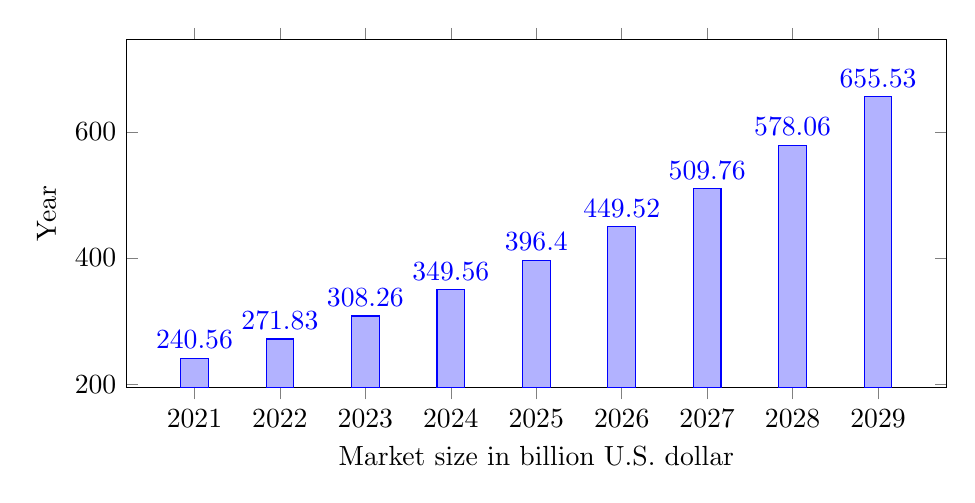
\begin{tikzpicture}
        \begin{axis}[
            ybar,
            %width=35pt
            height=6cm,
            width=12cm, 
            ymax=700,
            x tick label style={/pgf/number format/1000 sep=},
            ylabel=Year,
            xlabel=Market size in billion U.S. dollar,
            enlargelimits=0.1,
            %legend style={at={(0.5,-0.1)},
            %anchor=north,legend columns=-1}, 
            %ybar interval=0.4,
            nodes near coords,]
            \addplot coordinates { (2021,240.56) (2022,271.83) (2023,308.26) (2024,349.56) (2025,396.4) (2026,449.52) (2027,509.76) (2028,578.06) (2029,655.53)};
            %\addplot coordinates {(2012,388950) (2011,393007) (2010,398449) (2009,395972)};
            %\legend{Year}
        \end{axis}
    \end{tikzpicture}
    \caption[Big data analytics market size]{Size of the big data analytics market worldwide from 2021 to 2029 (\cite{statista.2022})}
    \label{fig:bigDataMarket}
\end{figure}

This new trend, often coined \enquote{big data} after the fact that never before seen amounts of data are generated and are available for processing, enables completely new business areas. This is reinforced, among other things, by the fact that many companies already view their data as a primary business asset (\cite{Redman.2008}). Simultaneously, the emergence of big data promises to completely reshape the decision-making process of traditional businesses through the adoption of data analytics. Although sales in the area of big data have risen significantly over the past years (\cite{BISResearch.2018}, \cite{Bitkom.2018}) and businesses already view big data as an important information technology trend (\cite{Bitkom.2017}) a lot of organizations struggle to effectivly utilize their data. Some 84\% of industry-leading companies in the United States and around the world were already investing in big data analytics in 2019, according to their own statements, which only underlines the importance of data analytics for decision-making in the economy. (\cite{statista.2019}). This is also reinforced by the market for big data analytics worlwide expected to more then double in size in the next 6 years (figure \ref{fig:bigDataMarket})\newline




\subsection{Applied \& Theoretical Research Problem} %and significance

In their article, Amankwah-Amoah and Adomako study the influence of big data usage on business failure. 
They come to the conclusion that the mere possession of big data as an asset has no positive effects on an organization (\cite{AmankwahAmoah.2019}) and that in order to prevent business failure, big data must be used effectively (\cite{AmankwahAmoah.2019}). Conducting research to resolve the underlying factors hindering the efficient utilization of data analytics in this particular context holds therefore crucial significance. However, although decision-making in data analytics has recently attracted scholars' attention (\cite{Chen.2022}) there is still a lack of research on non-technical aspects holding back the utilization of data analytics. Section \ref{sec:identification_of_the_problem} of this thesis uses the information-value-chain to look at the state of research in data analytics. Specifically, a literature review on Boundaries and Conflicts in the field of Data Analytics is conducted. The results of this literature review show that there is a lack of research on non-technical aspects on the information-value-chain. These literature gaps mainly consist of areas like decision-making and behavioral research. These results are confirmed by studies in the past (\cite{Trieu.2017}), which might indicate a persistant issues. This only becomes more apparent as new technologies, which overlap with data analytics like machine learning and artificial intelligence get more widespread. These \enquote{black-box}\footnote{Technologies whose exact internal sequence can hardly or not at all be explained, which therefore are acting like a \enquote{black-box}} technologies are already alternatives to human decision-making (\cite{Krakowski.2023}). Moreover other studies confirm that aspects like company culture, business models and the overall commitment and strategy of organizations have a big impact on the effectiveness of data analyitics (\cite{Holsapple.2014}). This lack of research on non technical regards could become a huge issue in the future, specifically for the decision-making process as firms' top priorities focus more and more on big data analytics for strategic decision making (\cite{Ghasemaghaei.2019}). 

Furthermore, it is indicated in section \ref{sec:identification_of_the_problem} that the current state of research specifically lacks a variety of experiments conducted to confirm the validity of frameworks and hypothesis. The experiment being a particularly important tool for investigating causal relationships in research (\cite{Gniewosz.2011}). In addition other means of collecting information like inquest questionnaires, which are probably the most frequently used form of obtaining information (\cite{Mummendey.2014}) in quantitative research are not always the most suitable method. The behavior of people, for example, which comprises the literature gap found, can be better assessed by means of observational studies or experiments (\cite{Gniewosz.2011}). While prior research has conducted behavioral research of data analytics with surveys and case studies, little or no attention has been paid to the verification of research results and hypothesis through experiments. This general lack of experimental research in certain areas connects the applied business problem of better utilizing data analytics to the theoretical problem of lack of experimental research generally found in data analytics (refering to the results of the literature search in section \ref{sec:identification_of_the_problem}). Improving the experimental research process in the field of data analytics could thereby significantly improve the future state of knowledge on said topic, whilste also allowing organizations to succeed in the fast paste economical environment of the digital-age.

%In summary, the topic of data analytics is extremely relevant in the current economic environment. Especially due to overlaps with Big Data and Artificial Intelligence as well as Machine Learning. Nonetheless, there are large research gaps in non-technical subfields complemented by a lack of experimental research.



%\subsection{Methodology and Scope of the Study}

\subsection{Objective and Expected Contribution}


The objective of this thesis is to improve the experimental research process in the field of behavioral research in data analytics. This is done through the following three objectives: (1) the review of prior research on data analytics and their methodological procedure (2) the development of an artefact which improves the research process in the field of behavioral research in data analytics (3) the validation of the artefact through the exemplary realization of a study in said field utilizing said artefact. In order to accomplishe the creation of this artefact the \ac{dsc} methodology is used. This methodology contains six steps, \textit{Identification of the Problem}, \textit{Definition of Objectives for a solution}, \textit{Design and Dev of artefacts}, \textit{Demonstration of the Artifact}, \textit{Evaluation of the solution} and \textit{Communication} (\cite{Peffers.2006}, \cite{Dresch.2015}). 
The \textit{identification of the problem} is conducted in section \ref{sec:identification_of_the_problem} through a literature search. To be more specific the current state of research in the field of boundaries and conflicts that limit the utilization of data analytics is investigates. As stated before this results in the identification of a gap in literature in the field of behavioral research in data analytics. After identifying the problem, the next step of the \ac{dsc} Methodology is the \textit{definition of objectives for a solution}. This is accomplished by specifying requirements for the final artifact using the current state of literature in data analytics and the \textit{requirement engineering} approach. For this purpose, a second literature search is utilized to identify literature in the field of data analytics that uses experiments or whose research object would in principle have permitted the use of experiments. These insights are then used to conceptualize, analyze and validate requirements for the final artefact (\cite{Sommerville.2011}, \cite(SWEBOK.2004)). %The \textit{Design and Dev of artefacts} step of the \ac{dsc} framework 
As the name of the next step suggests the artefact is designed and implemented in the \textit{design and dev of artefacts} phase using the requirements specified in the last step. Subsequently, the resulting artefact is then demonstrated in the \textit{Demonstration of the Artifact} step. The \textit{Evaluation of the solution} phase then implements a real experimental study in data analytics as an example to evaluate the artefact and its benefits for the experimental research process. This examplary implementation is then also used to validate the afformentioned requirements. The last step of the \ac{dsc} framework, which focusses on communicating the results to its stakeholders, is ensured by this thesis itself. 

The practical contribution of this thesis to research is twofold. On the one hand an artefact is created which accelerates research in the field of data analytics, through the improvement of the research process. On the other hand meta-knowledge about the research process itself is created, which not only improves the conduct of research through said artefact, but can also be used in off-topic areas beyond the use cases of this thesis.

In summation, the goal of this thesis is to develop an artifact that improves the experimental research process in behavioral research in data analytics. For this purpose, the \ac{dsc} method is used to create an artifact. The requirements for this artifact are established using past experimental and non-experimental studies in data analytics and the requirement engineering approach. The artifact is then validated by implementing a real study as an example, thereby demonstrating the improvements to the experimental behavioral research process in data analytics.




%and evaluation using the these requirements, in the \textit{Demonstration of the Artifact} and \textit{Evaluation of the solution} steps. The \textit{Demonstration of the Artifact} step serves as a general demonstration of the artefact where the \textit{Evaluation of the solution} phase 

%the exemplary implementation of a real experiment setup 

 %to develope a technical artefact as a solution for the afformentioned problem.  and \textit{Evaluation of the solution} steps. The last step of the \ac{dsc} framework, which focusses on communicating the results to its stakeholders, is ensured by this thesis itself. The last step is thus already fulfilled by this theis itself and will not be considered further.









%utilizes a second literature search to collect an detailed overview about what kind of studies have been conducted in the field of data analytics already, with a special focus on, whether these studies have used custom applications to conduct experiments. These findings are then used to develop requirements using the requirement engineering framework, which is in of itself made up of four different steps \textit{Elicit requirements}, \textit{Requirements specification}, \textit{Verification and validation} and \textit{Requirements management}. These requirements are then used in the 


%Although decision-making in data analytics has recently attracted scholars' attention (\cite{Pearson.1998}) there seems to be still a lack of research on the behavioral aspects of data analytics.

%This, however, might be hindered by boundaries and conflicts that have arisen during an organization's existence. Technical challenges are only some part of the underlying problem. 

%Any circumstance that prevents the effective use of data analytics therefore poses a real threat to a company's existence.

%Es wurde teilweise wenig geforscht, speziell wenig zu behavioral Aspekten
%In their article, Amankwah-Amoah and Adomako study the influence of big data usage on business failure. 
%They come to the conclusion that the mere possession of big data as an asset has no positive effects on an organization (\cite{AmankwahAmoah.2019}) and that in order to prevent business failure, big data must be used effectively (\cite{AmankwahAmoah.2019}). 



%conditions beyond technical aspects like company culture, business models and the overall commitment and strategy of organizations play a big role in the effectiveness of data analyitics (\cite{Holsapple.2014}). 



%Other conditions beyond technical aspects like company culture, business models and the overall commitment and strategy of organizations play a big role in the effectiveness of data analyitics (\cite{Holsapple.2014}). 

%Although many authors, such as C. Holsapple et. al, have already pointed out that non-technical factors have an influence on the effectiveness of data analytics (\cite{Holsapple.2014}), the current state of research still contains large gaps.


%Section \ref{sec:identification_of_the_problem} of this thesis uses the information-value-chain to look at the state of research in data analytics. Specifically, a literature review on Boundaries and Conflicts in the field of Data Analytics is conducted in this section. The results of this literature review show that there is a lack of research on non-technical aspects on the information-value-chain like decision-making and behavioral research. These results are confirmed by studies in the past (\cite{Trieu.2017}), which might indicate a persistant issues. This only becomes more apparent as new technologies which overlap with data analytics like machine learning and artificial intelligence get more widespread. These \enquote{black-box}\footnote{Technologies whose exact internal sequence can hardly or not at all be explained, which therefore are acting like a \enquote{black-box}} technologies are already alternatives to human decision-making (\cite{Krakowski.2023}), without their influence on organizations beyond technical aspects being properly researched. This could become a huge issues in the future as firms' top priorities focus more and more on big data analytics for strategic decision making (\cite{Ghasemaghaei.2019}).


%rely more and more on data analytics and other decision aid system for decision making (\cite{Chen.2022}). 

%Given this, many firms' top priorities have been the integration of digital technologies into existing business practices and the pplication of big data analytics (BDA) for strategic decision-making Ghasemaghaei.2019

%Although crisis decision-making has attracted scholars' attention 

%Although decision-making in data analytics has recently attracted scholars' attention (\cite{Pearson.1998}) there seems to be still a lack of research on the behavioral aspects of data analytics.

%often concidered to be the next big thing, are already gaining a lot of the attention in both research and businesses. Although these \enquote{black box} technologies are even less explainable than more traditional big data and data analytics frameworks, there is clear lack of research on their implementation in a non-technical sense. Should corporate executives blindly rely on data analytics and machine learning for their decision making process or just use them as a support tool? If a senior manager has a different opinion on a product release than what is specified by data analytics processes, who's opinion should be prioritized and to what extend? The technical basis for these technologies has in many cases been laid, but the question of how to behave in relation to these new technologies is yet to be answered most of the time

%Even though this fact is confirmed by multiple studies, there is still a lack in research on the utilization of data in organizations. In section  of this thesis 






%This fact which is confirmed in multiple studies.   


%Boundaries that have surfaced due to behavioral aspects regarding these new technologies might also impact the effective usage of data analytics. 



 %by researchers. %has not been resolved.

%Der Prozess der Forschung selbst kann sehr aufwendig und umständlich sein
%A lack of research in these areas can not only be attributed to these technologies being new. Answering these questions and conducting extensive research in this field can be expensive and time-consuming.

%Data-Value-Chain mit einbauen.

%While some areas of research can be easily conducted and are only limited by funding or the number of researchers, the area of data analytics 




%Not only results but the process of the research itself should be considered to fill possible gaps in the research on boundaries, conflicts and their use.

%In this context, dealing with these new technologies in a broader sense is just as big a challenge as technical aspects.

%regarding hindering boundaries and conflicts again focusses on the technology itself, rather than questioning the extent to which it should be used in the first place.

%the fact is taken into account that data analytics promises to reshape the decision-making process for whole industries without there being an appropriate level of behavioral research on these technologies. 

%not built around processing data, but have subsequently implemented some sort of data analytics system into their organization and processes.

%Many companies are at a point where they have a solid technical infrastructure and tools to deploy data analytics, but the decision-making process, use and day-to-day deployment of data analytics and how this technology should be handled in a wider sense is little questioned. This circumstance is further exacerbated by new trends which overlap with data analytics like machine learning and artificial intelligence. These technologies, often coined as the next big thing, are already gaining a lot of the attention in both research and businesses. Although these "black box" technologies are even less explainable than more traditional big data and data analytics technologies, much of the research regarding hindering boundaries and conflicts again focusses on the technology itself, rather than questioning the extent to which it should be used in the first place. Industries and researches are so focused on what these technologies can achieve that the question of whether it makes sense to use them at all, or to what extent, is not a priority. Should corporate executives blindly rely on data analytics and machine learning for their decision making process or just use them as a support tool? If a senior manager has a different opinion on a product release than what is specified by data analytics processes, who's opinion should be prioritized and to what extend? The technical basis for these technologies has been laid, but the question of how to behave in relation to these technologies has not been resolved.



%The reasons for these boundaries and conflicts that hinder the utilization of data analytics in organizations are not only limited to technical aspects, which concern the collection, processing and standardization of data, but also the handling of these new technologies in an overarching non-technical sense.
%While businesses already view big data as an important technology trend (\cite{Bitkom.2017}), there has been relatively little research done in the area of behavioral research. In the past couple of years this led many companies and researchers into spending an above-average share of resources into technical areas like data extraction, data preparation or data harmonization instead of researching the wider impact of data anyltics. While this has laid a solid foundation for the technology of data analytics itself, both in businesses and in research, it has also led to topics relating to the use and behavior of said technologies to being neglected. 
%In their article, Amankwah-Amoah and Adomako study the influence of big data usage on business failure. 
%They come to the conclusion that the mere possession of big data as an asset has no positive effects on an organization. In order to prevent business failure, big data must be used effectively  (\cite{AmankwahAmoah.2019}). 





%the decision-making process

%Looking at how companies utilize their available data an above-average share of resources is dedicatded to actions like data extraction or preparation, whilste areas beyond these more technical processes hardly get any attention. In the past couple of years this led to big investments 




%This thesis objective is to support the process of behavioral research in the field of data analytics. Due to the aforementioned reasons, an artefact is developed which can be used to conduct experiments in the field of data analytics with the focus of behavioral research. This artefact is supposed to streamline and cheapen research. 



%In summary the objective of this thesis is to develop a solution in the form of an artefact which enables researchers to design, conduct, and analyze studies more efficiently and cost-effectively, allowing them to explore the field of behavioral research in data analyitics in greater depth.


%Behavioral research can be conducted using a variety of quantitative and qualitative means. The experiment is probably the most time-consuming type of qualitative research, since it requires a great deal of time for the researcher to conduct and perform and a huge time commitment on the side of the participant. One of the major challenges in conducting expertiments in the area of data analytics is the high cost of developing custom applications. The development of such applications can be time-consuming, expensive, and often requires specialized expertise. Although there are already different applications for conducting studies of various kinds, such as survey tools, there is still a lack of applications that have been specifically developed to conduct behavioral research in the field of data analytics. Particularly there is a lack of applications that enable researchers to create studies on a wide range of use cases, without the need to develop tailor-made applications for each specific studies. %that are not tailor-mode for a specific study, but represent a more generic framework like approach that can be utilized in a variety of different studies.
%Moreover, follow-up research is made more difficult to conduct, as these custom applications are usually not publicly available and in most cases unflexible to customize for further studies. %Even if they are, it is to expected that these applications are very unflexible and would require a lot of investment to customize for slightly different use cases.
%Specifically, if a new application has to be created for each new study or follow up research, as these custom applications are usually not included in the publication of papers. 

%The communication of the results is ensured by this work itself.%, which is why no furhter measures are taken to communicate
    



%To address this challenge, this thesis sets out to develop a generic application that streamlines the process of conducting studies in the field of data analytics.


%\subsection{Contribution and Scope of the Study}

%This application enables researchers to design, conduct, and analyze studies more efficiently and cost-effectively, allowing them to explore the field in greater depth. This will be accomplished by using the \ac{dsc} approach. Firstly, the problem of a lack of behavioral research in data analytics is identified. Then, the objectives for a solution are defined through a literature review and the use of requirement engineering to gather requirements for the application. Next, the application is design, implemented prototypically and its functionality demonstrated. Finally, solution is evaluated through the usages of the requirements.

%The role of information systems in \ac{it} modern business solutions is indisputable, [...] Developing such a solution is the goal of %this work \parencite{venkatesh_usability_2014}. 

%Process mining needs to access [...] and used by many large-scale companies \parencite{hoehle_espoused_2015} across the world.

%And here we demonstrate like \parencite{hoehle_espoused_2015} how citations look alike in this \LaTeX file. You can also list all authors \parencite{venkatesh_usability_2014}. And click any of the references and see what happens in your PDF reader, like here: \textcite{university_of_arkansas_mobile_2015}.